\begin{figure}
	\centering
	\begin{subfigure}{0.48\linewidth}
		\centering
		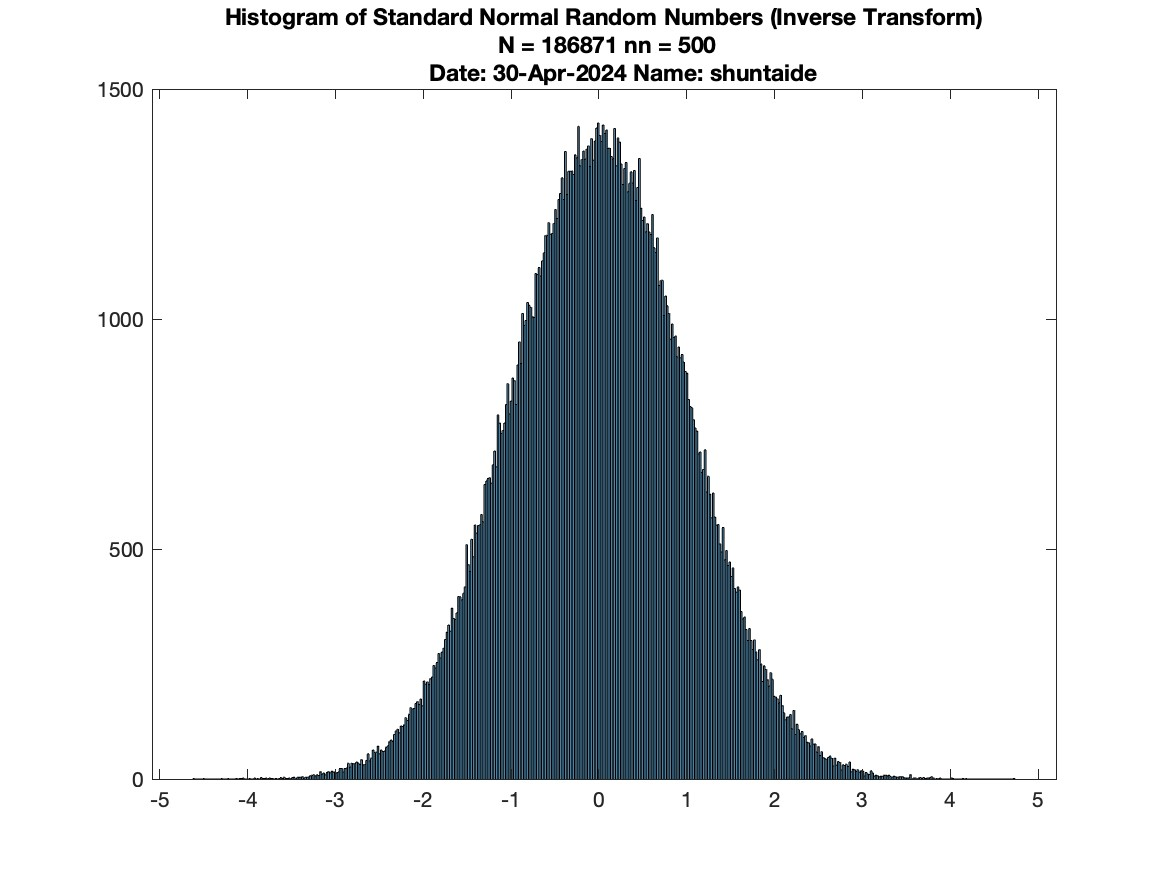
\includegraphics[width=0.8\linewidth]{src/figures/inverse-transform/Inverse_trans_hist_N=186871_nn=500.jpg}
		\subcaption{ヒストグラム}
	\end{subfigure}
	\begin{subfigure}{0.48\linewidth}
		\centering
		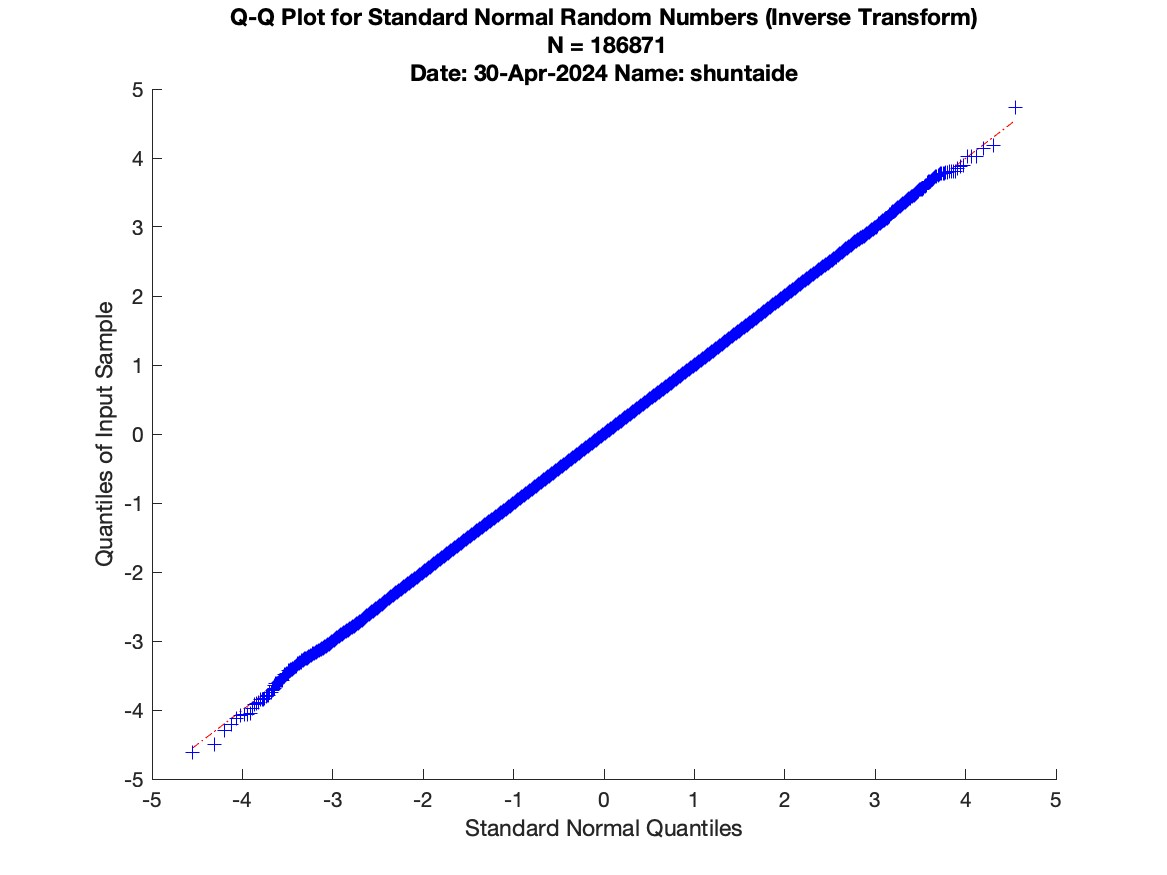
\includegraphics[width=0.8\linewidth]{src/figures/inverse-transform/Inverse_trans_qqpl_N=186871.jpg}
		\subcaption{QQプロット}
	\end{subfigure}
	\caption{逆変換法による標準正規乱数の生成結果}\label{fig:inverse-transform-random}
\end{figure}
